\chapter{Interpolation}

\section{Introduction}

\subsection{Definition}

\begin{example}
    Suppose we are given the following population data
    \begin{table}[H]
        \centering
        \begin{tabular}{r|c|c|c|c|c|c|c|c}
            year           & 1940 & 1950 & 1960 & 1970 & 1980 & 1990 & 2000 & 2010 \\
            \hline
            Population (M) & 132  & 151  & 179  & 203  & 226  & 249  & 281  & 308
        \end{tabular}
    \end{table}
    We mey ask the question: what was the population in 1965? We can use \term{interpolation} to estimate the population in 1985.

    \begin{figure}[H]
        \centering
        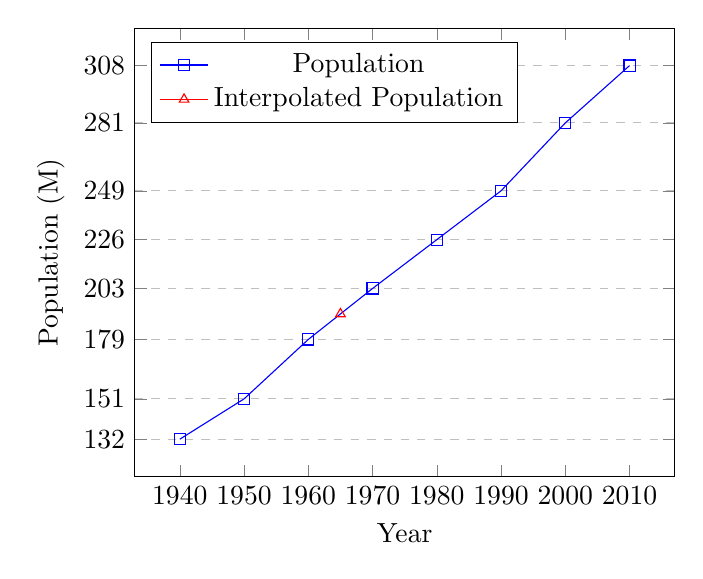
\begin{tikzpicture}
            \begin{axis}[
                    xlabel={Year},
                    ylabel={Population (M)},
                    xtick={1940, 1950, 1960, 1970, 1980, 1990, 2000, 2010},
                    ytick={132, 151, 179, 203, 226, 249, 281, 308},
                    xticklabel style={/pgf/number format/1000 sep=},
                    yticklabel style={/pgf/number format/1000 sep=},
                    legend pos=north west,
                    ymajorgrids=true,
                    grid style=dashed,
                ]

                \addplot[
                    color=blue,
                    mark=square,
                ]
                coordinates {
                        (1940, 132)
                        (1950, 151)
                        (1960, 179)
                        (1970, 203)
                        (1980, 226)
                        (1990, 249)
                        (2000, 281)
                        (2010, 308)
                    };
                \addlegendentry{Population}

                \addplot[
                    color=red,
                    mark=triangle,
                ]
                coordinates {
                        (1965, 191)
                    };
                \addlegendentry{Interpolated Population}

            \end{axis}
        \end{tikzpicture}
        \caption{Population data and interpolated population in 1965}
    \end{figure}

    We may also ask the question: what will the population be in 2020? This will be an \term{extrapolation} problem.
\end{example}

\begin{definition}
    Given a set of \( m \) data points \( \{ (t_i, y_i) \}_{i=1}^{m} \) with \( t_1 < t_2 < \cdots < t_m \), the \textbf{interpolation problem} is to find a function \( g(t) \) from a specific class of functions that \[
        g(t_i) = y_i \quad \text{for all } i = 1, 2, \ldots, m
    \]
\end{definition}

\begin{remark}
    Another use of interpolation is to approximate a function \( f(t) \) by a simpler function \( g(t) \) that is easier to work with.
\end{remark}

\begin{example}
    Suppose we have a function \[
        \operatorname{erf} = \frac{2}{\sqrt{\pi}} \int_{0}^{x} e^{-t^2} \, dt
    \] and we want to approximate it with a polynomial.
    \begin{itemize}
        \item Evaluate \( \operatorname{erf} \) at \( m \) points, \( \{ (x_i, e_i) \}_{i=1}^{m} \)
        \item Interpolate the points with a polynomial \( p(x) \) such that \( p(x_i) = e_i \) for all \( i = 1, 2, \ldots, m \)
        \item Use the interpolant \( p(x) \) in place of \( \operatorname{erf} \)
    \end{itemize}
\end{example}

\subsection{Design Goals for Interpolation}

\begin{enumerate}
    \item Easy to evaluate -- quick, accurate
    \item Gives accurate approximations for \( t \neq t_i \)
    \item Can integrate and differentiate easily
\end{enumerate}

\begin{remark}[Caveats]
    Interpolations come with some caveats.

    \begin{itemize}
        \item Interpolations are not uniques.
        \item Not all interpolations have nice properties
        \item Interpolations does not always give the right solution choice
    \end{itemize}
\end{remark}

\begin{note}
    We assume \textbf{accurate data} has the form \[ \{ (t_i, y_i) \}_{i=1}^m \qquad \text{ or } \qquad \{ t_i, f(t_i) \}_{i=1}^m \] with \[ t_1 < t_2 < \cdots < t_m \]
\end{note}

\subsection{Interpolation Problems}

\begin{example}
    Suppose we want to construct a linear fit for the data \[
        \{ (-1, 2), (1, 1) \}
    \]
    Define \( P_1(t) = b + mt \). We have \( \begin{cases} P_1(-1) = 2 \\ P_1(1) = 1 \end{cases} \implies \begin{cases} b + m (-1) = 2 \\ b + m (1) = 1 \end{cases} \) which yields the solution \[
        b = -\frac{1}{2} \qquad b = \frac{3}{3} \qquad \text{ so } \qquad P_1(t) = \frac{3}{2} - \frac{1}{2}t
    \]
\end{example}

\begin{example}
    Suppose we want to construct a quadratic fit for the data \[
        \{ (-1, 2), (1, 1), (2, 1) \}
    \]
    Define \( P_2(t) = a + bt + ct^2 \). We have \( \begin{cases} P_2(-1) = 2 \\ P_2(1) = 1 \\ P_2(2) = 1 \end{cases} \implies \begin{cases} a + b(-1) + c(-1)^2 = 2 \\ a + b(1) + c(1)^2 = 1 \\ a + b(2) + c(2)^2 = 1 \end{cases} \) which yields \[
        P_2(t) = \frac{4}{3} - \frac{1}{2}t + \frac{1}{6}t^2
    \]
\end{example}

\begin{note}
    We choose polynomial interpolants \[
        P_{m-1}(t) = \sum_{i=1}^m c_i t^{i-1}
    \] because they are easy to evaluate. The operation count is approximately \[
        3n \text{ FLOPs}
    \]
\end{note}

\begin{theorem}[Horner's Rule]
    We can re-write our polynomial as \[
        P_{m-1}(t) = c_1 + t(c_2 + t(c_3 + t(\cdots + t(c_{m-1} + c_m t))))
    \]
\end{theorem}

\begin{note}
    Horner's methods provide some advantages. The operation count reduces to \[
        2m \text{FLOPs}
    \] and it's easier to integrate and differentiate.
\end{note}

\begin{theorem}
    For a set of points \[
        \{ (t_i, y_i) \}_{i=1}^m,
    \] there exists a unique polynomial of degree at less than \( m \) that interpolates the data.
\end{theorem}

\section{Solving Interpolation Problems}

\subsection{Monomial Basis}

Given a set of points \[
    S = \{ (t_i, y_i) \}_{i=1}^m
\] we find the unique polynomial \[
    P_{m-1}(t) = \sum_{i=1}^{m} c_i t^{i-1}
\] that interpolates the data.

Applying the interpolation conditions,
\begin{itemize}
    \item \( P_{m-1}(t_1) = y_1 \)
    \item \( P_{m-1}(t_2) = y_2 \)
    \item \( \vdots \)
    \item \( P_{m-1}(t_m) = y_m \)
\end{itemize}
We have systems of equations
\begin{align*}
    c_1 + c_2 t_1 + c_3 {t_1}^2 + \cdots + c_m {t_1}^{m-1} & = y_1 \\
    c_1 + c_2 t_2 + c_3 {t_2}^2 + \cdots + c_m {t_2}^{m-1} & = y_2 \\
    \vdots                                                         \\
    c_1 + c_2 t_m + c_3 {t_m}^2 + \cdots + c_m {t_m}^{m-1} & = y_m
\end{align*}
That is, a linear system \[
    \begin{pmatrix}
        1      & t_1    & t_1^2  & \cdots & {t_1}^{m-1} \\
        1      & t_2    & t_2^2  & \cdots & {t_2}^{m-1} \\
        \vdots & \vdots & \vdots & \ddots & \vdots      \\
        1      & t_m    & t_m^2  & \cdots & {t_m}^{m-1}
    \end{pmatrix} \begin{pmatrix}
        c_1    \\
        c_2    \\
        \vdots \\
        c_m
    \end{pmatrix} = \begin{pmatrix}
        y_1    \\
        y_2    \\
        \vdots \\
        y_m
    \end{pmatrix}
\]

The matrix \( V \) is called the \term{Vandermonde matrix}.

\begin{lemma}
    If all the \( t_i \) are distinct, then the Vandermonde matrix is invertible.
\end{lemma}

Therefore, we can determine the poly coefficients \( \vec{c} \).

\begin{minted}{python}
    import numpy as np

    t = np.linspace(1.0, 2.0, 11)
    # t = (1.0, 1.1, 1.2, ..., 2.0)

    V = np.vander(t, increasing=True)
    # V = [[1.0, 1.0, 1.0, ..., 1.0],
    #      [1.0, 1.1, 1.21, ..., 2.0],
    #      ...
    #      [1.0, 2.0, 4.0, ..., 1024.0]]

    np.linalg.cond(V)
    # 6518493762298.583 ~ 6.52 * 10^12
\end{minted}

Using IEEE double precision, solving \( V \vec{c} = \vec{y} \) get \( \vec{c}'s \) to approximately 4 significant digits of accuracy. It is difficult to determine interpolants accurately this way.

Originally, we are trying to find \( P_{m-1}(t) \in \P_{m-1} \), write \[
    P_{m-1}(t) = \sum_{i=1}^{m} c_i t^{i-1}
\] using monomial basis \[
    \{ 1, t, t^2, \ldots, t^{m-1} \}
\]

\subsection{Lagrange Basis}

\subsubsection{Using a Different Basis}
Suppose \( \{ b_i(t) \}_{i=1}^{m} \) is a basis for \( \P_{m-1} \), then \[
    P_{m-1}(t) = \sum_{i=1}^{m} \alpha_i b_i(t)
\] for some \( \alpha_i \in \R \) to be determined.

We know that \[
    P_{m-1}(t_i) = y_i
\] and using the new basis, we have
\begin{align*}
    \alpha_1 b_1(t_1) + \alpha_2 b_2(t_1) + \cdots + \alpha_m b_m(t_1)
     & = y_1  \\
    \alpha_1 b_1(t_2) + \alpha_2 b_2(t_2) + \cdots + \alpha_m b_m(t_2)
     & = y_2  \\
     & \vdots \\
    \alpha_1 b_1(t_m) + \alpha_2 b_2(t_m) + \cdots + \alpha_m b_m(t_m)
     & = y_m
\end{align*} which yields the system of equations \[
    \begin{pmatrix}
        b_1(t_1) & b_2(t_1) & \cdots & b_m(t_1) \\
        b_1(t_2) & b_2(t_2) & \cdots & b_m(t_2) \\
        \vdots   & \vdots   & \ddots & \vdots   \\
        b_1(t_m) & b_2(t_m) & \cdots & b_m(t_m)
    \end{pmatrix} \begin{pmatrix}
        \alpha_1 \\
        \alpha_2 \\
        \vdots   \\
        \alpha_m
    \end{pmatrix} = \begin{pmatrix}
        y_1    \\
        y_2    \\
        \vdots \\
        y_m
    \end{pmatrix}
\]

\begin{remark}
    The choice of basis is important. We want to choose a basis that is easy to work with.
\end{remark}

What if \( B = I \)? Then we \( \kappa_I = 1 \) and \( \vec{\alpha} = \vec{y} \).

We choose a basis such that \[
    b_i(t_j) = \begin{cases}
        1 & \text{if } i = j    \\
        0 & \text{if } i \neq j
    \end{cases}
\]

\begin{example}
    Consider \( R = 1 \), we want
    \begin{itemize}
        \item \( b_1 (t_2) = 0 \)
        \item \( b_1 (t_3) = 0 \)
        \item \( \vdots \)
        \item \( b_1 (t_m) = 0 \)
    \end{itemize}

    So if we were to construct a polynomial satisfying these conditions, we would include the factors \[
        (t - t_2) \qquad (t - t_3) \qquad \cdots \qquad (t - t_m)
    \] which suggests \( b_1(t) \) takes the form \[
        (t - t_2)(t - t_3) \cdots (t - t_m)
    \]

    Note that this is of degree \( m-1 \), and since our basis cannot have degree more than \( m-1 \), we cannot add more factors.

    Now we need to satisfy \( b_1(t_1) = 1 \), so we need to divide by a constant. We can choose \[
        b_1(t) = \frac{(t - t_2)(t - t_3) \cdots (t - t_m)}{(t_1 - t_2)(t_1 - t_3) \cdots (t_1 - t_m)}
    \]
\end{example}

In general, \[
    b_k(t) = \frac{\displaystyle\prod_{j=1, j \neq k}^{m} (t - t_j)}{\displaystyle\prod_{j=1, j \neq k}^{m} (t_k - t_j)}
\]

\begin{lemma}
    The set of functions \[
        \{ {b_k}(t) \}_{k=1}^{m}
    \] are linearly independent and form a basis for \( \P_{m-1} \).
\end{lemma}

This basis is know as the \term{Lagrange basis}.

\begin{definition}[Lagrange Basis]\index{Lagrange Basis}
    The \textbf{Lagrange basis} is a set of functions \[
        \{ l_k(t) \}_{k=1}^{m} \qquad \text{where} \qquad l_k(t) =
        \prod_{j=1, j \neq k}^{m} \frac{t - t_j}{t_k - t_j}
    \]
\end{definition}

\begin{remark}
    The Lagrange basis has the property \[
        l_k(t_j) = \begin{cases}
            1 & \text{if } k = j    \\
            0 & \text{if } k \neq j
        \end{cases}
    \]
\end{remark}

The Lagrange form of the interpolating polynomial is \[
    P_{m-1}(t) = \sum_{k=1}^{m} c_k l_k(t) \qquad\text{ where } \vec{c} = \vec{y}
\]

\begin{example}
    We use the Lagrange basis to compute \( P_2(t) \) that interpolates \[
        \{ (-1, 2), (1, 1), (2, 1) \}
    \]

    We have the expressions for the Lagrange basis

    \begin{minipage}[t]{0.3\linewidth}
        \begin{align*}
            l_1(t)
             & = \prod_{k=2,3} \frac{t - t_k}{t_1 - t_k}
            \\
             & = \frac{t - 1}{-1 - 1} \cdot \frac{t - 2}{-1 - 2}
            \\
             & = \frac{1}{6} (t - 1)(t - 2)
        \end{align*}
    \end{minipage}
    \begin{minipage}[t]{0.3\linewidth}
        \begin{align*}
            l_2(t)
             & = \prod_{k=1,3} \frac{t - t_k}{t_2 - t_k}
            \\
             & = \frac{t + 1}{1 + 1} \cdot \frac{t - 2}{1 - 2}
            \\
             & = -\frac{1}{2} (t + 1)(t - 2)
        \end{align*}
    \end{minipage}
    \begin{minipage}[t]{0.3\linewidth}
        \begin{align*}
            l_3(t)
             & = \prod_{k=1,2} \frac{t - t_k}{t_3 - t_k}
            \\
             & = \frac{t + 1}{2 + 1} \cdot \frac{t - 1}{2 - 1}
            \\
             & = \frac{1}{3} (t + 1)(t - 1)
        \end{align*}
    \end{minipage}

    so \begin{align*}
        P_2(t)
         & = 2l_1(t) + 1l_2(t) + 1l_3(t)
        \\
         & = 2 \cdot \frac{1}{6} (t - 1)(t - 2) - \frac{1}{2} (t + 1)(t - 2) + \frac{1}{3} (t + 1)(t - 1)
        \\
         & = \frac{4}{3} - \frac{1}{2}t + \frac{1}{6}t^2
    \end{align*}
    which is the same as the polynomial we found earlier.
\end{example}

\begin{remark}[Lagrange Basis are Expensive]
    For each \( l_i(t) \), we require approximately \( 4m \) FLOPs.
    \begin{itemize}
        \item For the numerator, \( m - 1 \) multiplications and \( m - 1 \) subtractions
        \item For the denominator, \( m - 1 \) multiplications and \( m - 1 \) subtractions
        \item A finial division
    \end{itemize} so we require a total of \[
        \Theta(m^2) \text{ FLOPs}
    \] in total to compute the Lagrange basis.
\end{remark}

\subsection{Newton Basis}

Recall for a general basis \( \{ b_i(t) \}_{i=1}^{m} \), we have \[
    P_{m-1}(t) = \sum_{i=1}^{m} \alpha_i b_i(t)
\] and the interpolating conditions \[
    P_{m-1}(t_i) = y_i
\] We solve the system of equations \[
    B\vec{c} = \vec{y}
\] for \( \vec{c} \), where \[
    B = \begin{pmatrix}
        b_1(t_1) & b_2(t_1) & \cdots & b_m(t_1) \\
        b_1(t_2) & b_2(t_2) & \cdots & b_m(t_2) \\
        \vdots   & \vdots   & \ddots & \vdots   \\
        b_1(t_m) & b_2(t_m) & \cdots & b_m(t_m)
    \end{pmatrix}
\]

We want a \( B \) that is easy to solve, but perhaps not as easy as the identity matrix. We explore a triangular system.

\subsubsection{Lower Triangular System}

We choose a basis \( \{ b_i(t) \}_{i=1}^{m} \) such that \[
    B = \begin{pmatrix}
        b_1(t_1)     & 0            & 0      & \cdots           & 0        \\
        b_1(t_2)     & b_2(t_2)     & 0      & \cdots           & 0        \\
        \vdots       & \vdots       & \ddots & \ddots           & \vdots   \\
        b_1(t_{m-1}) & b_2(t_{m-1}) & \cdots & b_{m-1}(t_{m-1}) & 0        \\
        b_1(t_m)     & b_2(t_m)     & \cdots & b_{m-1}(t_m)     & b_m(t_m)
    \end{pmatrix}
\]

For simplicity, take \( b_1(t) = 1 \).
\begin{itemize}
    \item Row 1: \( b_2(t_1) = 0, b_3(t_1) = 0, \ldots, b_m(t_1) = 0 \)

          We include \( (t - t_1) \) as a factor of each \( b_R(t) \) for \( R = 2, 3, \ldots, m \).

    \item Row 2: \( b_3(t_2) = 0, b_4(t_2) = 0, \ldots, b_m(t_2) = 0 \)

          We include \( (t - t_2) \) as a factor of each \( b_R(t) \) for \( R = 3, 4, \ldots, m \).

    \item \( \vdots \)

    \item Row \( m-1 \): \( b_m(t_{m-1}) = 0 \)

          We include \( (t - t_{m-1}) \) as a factor of \( b_m(t) \).
\end{itemize} which suggests \[
    b_k(t) = \prod_{j=1}^{k-1} (t - t_j)
\]

\begin{remark}
    This is a basis because we have \( m \) linearly independent functions.
\end{remark}

\begin{definition}[Newton Basis]\index{Newton Basis}
    The \term{Newton basis} is a set of functions \[
        \{ n_k(t) \}_{k=1}^{m} \qquad \text{where} \qquad n_k(t) = \prod_{j=1}^{k-1} (t - t_j)
    \]
\end{definition}

The Newton form of the interpolating polynomial is \[
    P_{m-1}(t) = \sum_{k=1}^{m} c_k \prod_{j=1}^{k-1} (t - t_j)
\]

\begin{remark}[Newton Basis are Cheaper]
    If we can remember the results \( t - t_i \), then each new term added would only require \( 3 \) FLOPs. This is a significant improvement over the Lagrange basis. The total operation count is \(
        \Theta(3m) \text{ FLOPs}
    \)
\end{remark}

Now, to determine the coefficients, we solve a lower triangular system \( B\vec{c} = \vec{y} \)
We know that
\begin{itemize}
    \item \( y_1 = P_{m-1}(t_1) = c_1 \) so \[
              c_1 = y_1
          \]
    \item \( y_2 = P_{m-1}(t_2) = c_1 + c_2(t_2 - t_1) \) so \[
              c_2 = \frac{y_2 - c_1}{t_2 - t_1}
          \]
    \item \( \vdots \)
    \item \( \displaystyle y_m = P_{m-1}(t_m) = \sum_{k=1}^{m} c_k \prod_{j=1}^{k-1} (t_m - t_j) \) so \[
              c_m = \frac{\displaystyle y_m - \sum_{j=1}^{m-1} c_j \prod_{k=1}^{j-1} (t_m - t_k)}{\displaystyle \prod_{k=1}^{m-1} (t_m - t_k)}
          \]
\end{itemize}